\documentclass[12pt]{article}
\usepackage{amssymb}
\usepackage{amsmath}
\usepackage{graphicx}
\usepackage{color}
\usepackage{geometry}
 \geometry{
 a4paper,
 total={210mm,297mm},
 left=20mm,
 right=20mm,
 top=20mm,
 bottom=20mm,
}
\usepackage[parfill]{parskip}
\usepackage[colorlinks=true]{hyperref}
\hypersetup{urlcolor=blue, citecolor=red}

\newtheorem{theorem}{Theorem}
\newtheorem{definition}{Definition}
\newtheorem{lemma}[theorem]{Lemma}
\newtheorem{rem}[theorem]{Remark}
\newtheorem{pro}[theorem]{Proposition}
\newtheorem{con}[theorem]{Conjecture}

\renewcommand{\vec}[1]{\ensuremath{\overrightarrow{#1}}}

\begin{document}
\begin{center}
{\huge \bf Idealized 2 links} \\
\end{center}
\vspace{1ex}
\begin{flushright}
Ferenc A. Bartha\\
fab2@rice.edu
\end{flushright}

\subsection*{Generalized Coordinates}
We use the following coordinates and notation:
\begin{itemize}
 \item The middle mass point is given in polar coordinates w.r. to the origin and the fixed $x$-, $y$-axes.
 \begin{itemize}
  \item the connection to the origin (fixed) is a weightless rod,
  \item the weight of the mass point is $m_1$,
  \item radius$\, = d_1$, constant,
  \item angle from $x$-axis to the direction $\vec{e_{r_1}} = \theta_1$.
 \end{itemize}
 \item The upper mass point is given in polar coordinates w.r. to middle point
 \begin{itemize}
  \item the connection to the middle point is a weightless rod,
  \item the weight of the mass point is $m_2$,
  \item radius$\, = d_2$, constant,
  \item angle from the direction $\vec{e_{r_1}}$ to the direction $\vec{e_{r_2}} = \theta_2$.
 \end{itemize}
 \item Consequently, we describe our system by $\theta_1$ and $\theta_2$ and their derivatives.
\end{itemize}

\begin{figure}[!ht]
	\centering
	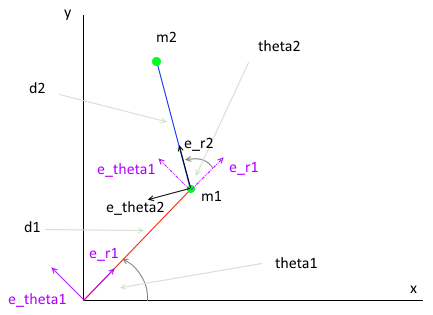
\includegraphics[scale=0.8]{01_Idealized_2links.png}
    \caption{The coordinates}
\end{figure}

Note that none of these coordinate systems (describing the middle or the upper point) is an inertial coordinate system. Both are rotating (thus accelerating) compared to the one fixed in the origin with axis $x$ and $y$.

\newpage

\subsection*{The Lagrangian}
We assume that no external forces act on the system, so we have conservation of energy, that is in our case conservation of kinetic energy.
The Lagrangian is
$$\mathcal{L}(\theta_1, \dot \theta_1, \theta_2, \dot \theta_2) = \frac{1}{2} m_1 |\vec{v_1}|^2 + \frac{1}{2} m_2 |\vec{v_2}|^2.$$
\vspace{1ex}
\noindent
We have
\begin{itemize}\itemsep 0.7ex
 \item conservation of energy: $\mathcal{L} = $ constant,
 \item the position vector of the middle mass from the origin is $d_1 \vec{e_{r_1}}$,
 \item the velocity vector is the derivative $\vec{v_1} = \dot{d_1} \vec{e_{r_1}} + d_1 \dot{\vec{e_{r_1}}} = d_1 \dot{\theta_1} \vec{e_{\theta_1}}$\\
 as $\dot d_1 = 0$ and $\dot{\vec{e_{r_1}}} = \dot{\theta_1} \vec{e_{\theta_1}}$ (see {\bf Appendix}),
 \item thus, the speed$^2$ is $|\vec{v_1}|^2 = (d_1 \dot{\theta_1})^2$,
 \item the position vector of the upper mass from the origin is $d_1 \vec{e_{r_1}} + d_2 \vec{e_{r_2}}$,
 \item the velocity vector is $\vec{v_2} = \vec{v_1} + \dot{d_2} \vec{e_{r_2}} + d_2 \dot{\vec{e_{r_2}}} = d_1 \dot{\theta_1} \vec{e_{\theta_1}} + d_2 (\dot{\theta_1} + \dot{\theta_2}) \vec{e_{\theta_2}}$\\
 as $\dot d_2 = 0$ and $\dot{\vec{e_{r_2}}} = (\dot{\theta_1} + \dot{\theta_2}) \vec{e_{\theta_2}}$  (see {\bf Appendix}),
 \item thus, the speed$^2$ is $|\vec{v_2}|^2 = (d_1 \dot{\theta_1})^2 + (d_2 (\dot{\theta_1} + \dot{\theta_2}))^2 + 2 d_1 d_2 \dot{\theta_1} (\dot{\theta_1} + \dot{\theta_2}) \mathrm{cos}(\mathrm{angle}(\vec{e_{\theta_1}}, \vec{e_{\theta_2}}))$\\
 that is $|\vec{v_2}|^2 = (d_1 \dot{\theta_1})^2 + (d_2 (\dot{\theta_1} + \dot{\theta_2}))^2 + 2 d_1 d_2 \dot{\theta_1} (\dot{\theta_1} + \dot{\theta_2}) \mathrm{cos}\theta_2$.
\end{itemize}

\vspace{1ex}
Thus, 
\begin{equation*}
\begin{split}
\mathcal{L}(\theta_1, \dot \theta_1, \theta_2, \dot \theta_2) = &\,\frac{1}{2} (m_1 + m_2) d_1^2 \dot{\theta_1}^2 
             + \frac{1}{2} m_2 d_2^2 (\dot{\theta_1} + \dot{\theta_2})^2
             + m_2 d_1 d_2 \dot{\theta_1} (\dot{\theta_1} + \dot{\theta_2}) \mathrm{cos}\theta_2.
\end{split}
\end{equation*}

\subsection*{Equations of Motion}
The equations of motion are derived by taking\\ {\it(Lagrange equations of the $2nd$ kind a.k.a Euler--Lagrange equations)}
$$d/dt [ \partial\mathcal{L}/\partial \dot q_j ] = \partial\mathcal{L}/\partial q_j$$
for all generalized coordinates $q_j \in \{\theta_1, \theta_2 \}$.

This gives us
$$\frac{d}{dt}\left[(m_1 + m_2) d_1^2 \dot{\theta_1} 
             + m_2 d_2^2 (\dot{\theta_1} + \dot{\theta_2})
             + m_2 d_1 d_2 (2 \dot{\theta_1} + \dot{\theta_2}) \mathrm{cos}\theta_2\right] = 0 \quad \text{ for } q_j = \theta_1$$
and
\begin{equation*}
 \frac{d}{dt}\left[m_2 d_2^2 (\dot{\theta_1} + \dot{\theta_2})
             + m_2 d_1 d_2 \dot{\theta_1} \mathrm{cos}\theta_2 \right] = 
  - m_2 d_1 d_2 \dot{\theta_1} (\dot{\theta_1} + \dot{\theta_2}) \mathrm{sin}(\theta_2) \quad \text{ for } q_j = \theta_2.
\end{equation*}

Writing in the time derivatives we get
\begin{equation*}
\begin{split}
  (m_1 + m_2) d_1^2 \ddot{\theta_1} 
 + m_2 d_2^2 (\ddot{\theta_1} + \ddot{\theta_2})
 + m_2 d_1 d_2 [(2 \ddot{\theta_1} + \ddot{\theta_2}) \mathrm{cos}\theta_2 - (2 \dot{\theta_1} + \dot{\theta_2})\dot{\theta_2} \mathrm{sin}\theta_2] = 0
\end{split}
\end{equation*}
that results in 
\begin{equation}\label{eq-theta1}
\begin{split}
 \left( m_2 d_2^2 + m_2 d_1 d_2 \mathrm{cos}\theta_2 \right) \ddot{\theta_2} = 
 &- \left( (m_1 + m_2) d_1^2 + m_2 d_2^2 + 2 m_2 d_1 d_2 \mathrm{cos}\theta_2 \right) \ddot{\theta_1}\\ 
 &+ m_2 d_1 d_2 (2 \dot{\theta_1} + \dot{\theta_2}) \dot{\theta_2} \mathrm{sin}\theta_2 
 \qquad \qquad \qquad \text{ for } q_j = \theta_1
\end{split}
\end{equation}
and
\begin{equation*}
 m_2 d_2^2 (\ddot{\theta_1} + \ddot{\theta_2})
 + m_2 d_1 d_2 [\ddot{\theta_1} \mathrm{cos}\theta_2 - \dot{\theta_1} \dot{\theta_2} \mathrm{sin}\theta_2] =
- m_2 d_1 d_2 \dot{\theta_1} (\dot{\theta_1} + \dot{\theta_2}) \mathrm{sin}(\theta_2)
\end{equation*}
that is transformed to
$$m_2 d_2^2 \ddot{\theta_2} =
- m_2 d_2^2 \ddot{\theta_1} - m_2 d_1 d_2 \ddot{\theta_1} \mathrm{cos}\theta_2 
- m_2 d_1 d_2 \dot{\theta_1}^2 \mathrm{sin}(\theta_2)
$$
and simplified to 
\begin{equation}\label{eq-theta2}
 \ddot{\theta_2} = - \left( \left[ 1 + \frac{d_1}{d_2} \mathrm{cos}\theta_2 \right] \ddot{\theta_1} + 
 \frac{d_1}{d_2} \dot{\theta_1}^2 \mathrm{sin}(\theta_2) \right)
  \qquad \qquad \qquad \qquad \text{ for } q_j = \theta_2
\end{equation}

\subsection*{Further Transformation of the Equations of Motion}
We want to solve the equations \eqref{eq-theta1} and \eqref{eq-theta2} for 
$\ddot{\theta_1}$ and $\ddot{\theta_1}$  
(some tools can model them as they readily are, but we need now a more standard form).

Substituting \eqref{eq-theta2} into \eqref{eq-theta1} yields
\begin{equation*}
\begin{split}
 - \left( m_2 d_2^2 + m_2 d_1 d_2 \mathrm{cos}\theta_2 \right) &\left( \left[ 1 + \frac{d_1}{d_2} \mathrm{cos}\theta_2 \right] \ddot{\theta_1} + \frac{d_1}{d_2} \dot{\theta_1}^2 \mathrm{sin}(\theta_2) \right) = \\
  &- \left( (m_1 + m_2) d_1^2 + m_2 d_2^2 + 2 m_2 d_1 d_2 \mathrm{cos}\theta_2 \right) \ddot{\theta_1}\\ 
 &+ m_2 d_1 d_2 (2 \dot{\theta_1} + \dot{\theta_2}) \dot{\theta_2} \mathrm{sin}\theta_2 
\end{split}
\end{equation*}
that is transformed to
\begin{equation*}
\begin{split}
 \big( m_1 d_1^2 + m_2 d_1^2 -& m_2 d_1^2 \mathrm{cos}^2\theta_2 \big) \ddot{\theta_1} =\\
 & m_2 d_1 d_2 (2 \dot{\theta_1} + \dot{\theta_2}) \dot{\theta_2} \mathrm{sin}\theta_2 
 + \left( m_2 d_2^2 + m_2 d_1 d_2 \mathrm{cos}\theta_2 \right) \frac{d_1}{d_2} \dot{\theta_1}^2 \mathrm{sin}(\theta_2)
\end{split}
\end{equation*}
and simplified to
\begin{equation}\label{eq-theta1b}
 \left( \tfrac{m_1}{m_2} + \mathrm{sin}^2\theta_2 \right) \ddot{\theta_1} =
  \tfrac{d_2}{d_1} (2 \dot{\theta_1} + \dot{\theta_2}) \dot{\theta_2} \mathrm{sin}\theta_2 
 + \left( \tfrac{d_2}{d_1} + \mathrm{cos}\theta_2 \right) \dot{\theta_1}^2 \mathrm{sin}(\theta_2)
\end{equation}

Substitute $\ddot{\theta_1}$ from \eqref{eq-theta1b} into \eqref{eq-theta2} and we reach the desired form.

\subsection*{Deriving the Initial Conditions}
Our experiment is the following. The initial alignment is $\theta_1(0) = \frac{\pi}{2}$ and $\theta_2(0) = 0$. A momentary impulse gives velocity to the middle point and does not affect the upper point.
\begin{itemize}
 \item $\vec{v_1}_{, init} = \vec{v_1}(0) = d_1 \dot{\theta_1}(0) \vec{e_{\theta_1}}(0)$ \\
 \hspace*{0.5cm} $\Rightarrow$ we obtain the initial value $\dot{\theta_1}(0)$.
 
 \item The upper point is not affected that is $\vec{0} = \vec{v_2}(0) = d_1 \dot{\theta_1}(0) \vec{e_{\theta_1}}(0) + d_2 (\dot{\theta_1}(0) + \dot{\theta_2}(0)) \vec{e_{\theta_2}}(0)$\\
 \hspace*{0.5cm} $\Rightarrow$ we obtain the initial value $\dot{\theta_2}(0) = - \frac{d_1}{d_2} \dot{\theta_1}(0) - \dot{\theta_1}(0)$\\
 \hspace*{1.1cm} as $\vec{e_{\theta_1}}(0) = \vec{e_{\theta_2}}(0)$ due to the initial alignment.
\end{itemize}

Recall that $\dot\theta_2$ is a relative coordinate with respect to the middle point that is in motion at time $0$. 
Thus, as the upper point is not in motion viewing from the fixed coordinate system centered at the origin, it is moving 
when viewed from the middle point, therefore, it has nonzero {\bf relative} velocity $d_2 (\dot{\theta_1}(0) + \dot{\theta_2}(0)) \vec{e_{\theta_2}}(0) = - d_1 \dot{\theta_1}(0) \vec{e_{\theta_2}}(0) = - d_1 \dot{\theta_1}(0) \vec{e_{\theta_1}}(0) = - \vec{v_1}(0)$.

\newpage
\subsection*{Appendix}
The derivation for $\dot{\vec{e_{r_1}}}(t) = \dot{\theta_1}(t) \vec{e_{\theta_1}}(t)$ is pretty straightforward. Centered at the origin, 
$\vec{e_{r_1}}(t)$ and $\vec{e_{\theta_1}}(t)$ form a coordinate system that rotates with speed $\dot{\theta_1}(t)$ around the origin 
(thus, rotates with respect to the inertial coordinate system). This rotation is actually around the $z$-axis (lifting it into 3D).

Given a position vector $\vec{p}_{relative}(t)$ of a moving point in this rotating coordinate system, its velocity (within this rotating system) is $\dot{\vec{p}}_{relative}(t)$. Looking from the origin in the inertial coordinate system, the effect of the rotation needs to be taken into account:
$$\dot{\vec{p}}_{global}(t) = \dot{\vec{p}}_{relative}(t) + \dot\theta_1(t) \vec{k} \times \vec{p}_{global}(t).$$
Here $\vec{k}$ is the axis of rotation, the direction of the $z$-axis.

Applying this for $\vec{p}_{global}(t) = \vec{e_{r_1}}(t)$, we get 
$$\dot{\vec{e_{r_1}}}(t) = \dot{(1,0)} + \dot\theta_1(t) \vec{k} \times \vec{e_{r_1}}(t) = \dot\theta_1(t) \vec{k} \times \vec{e_{r_1}}(t).$$
Now as $\vec{e_{\theta_1}}(t) = \vec{k} \times \vec{e_{r_1}}(t)$ by definition, we have shown the sought relation.

\vspace{1cm}
Similar argument works for $\dot{\vec{e_{r_2}}}(t) = (\dot{\theta_1}(t) + \dot{\theta_2}(t)) \vec{e_{\theta_2}}(t)$ as well. 
Translate $\dot{\vec{e_{r_2}}}(t)$ to the origin and observe that it actually rotates with speed 
$(\dot{\theta_1}(t) + \dot{\theta_2}(t))$ around the $z$-axis.

\subsection*{Further reading}
\begin{itemize}
 \item \href{http://en.wikipedia.org/wiki/Lagrangian_mechanics#Euler.E2.80.93Lagrange_equations}{Wikipedia - Lagrangian Mechanics}
 \item \href{http://ocw.mit.edu/courses/aeronautics-and-astronautics/16-07-dynamics-fall-2009/lecture-notes/MIT16_07F09_Lec08.pdf}{MIT OpenCourseware - Dynamics - Relative Motion using Rotating Axis}
 \item \href{http://en.wikibooks.org/wiki/Kinematics/2D_Coordinate_Systems}{Wikibooks - 2D Coordinate Systems}
 \item \href{http://en.wikipedia.org/wiki/Double_pendulum}{Wikipedia - Double Pendulum}
\end{itemize}
\end{document}

